\section{Felder}
\subsection{Das elektrische Feld, Elektrostatik}
Elektrostatik: Lehre von den ruhenden elektrischen Ladungen und deren Wirkung auf ihre Umgebung, insbesondere auf andere Ladungen\\
\subsubsection{Was ist ein Feld? Eigenschften, Darstellung}
\textbf{Feld}:Zustand des Raumes, bei dem jedem Punkt innerhalb eines bestimmten Gebietes eine physikalische Grösse - die Feldgrösse - zugeordnet ist.\\
Ein Feld ist eine 2D Fläche mit der Länge l und der Breite b.\\
Die Feldgrösse, z.B. Temperatur oder Geschwindigkeit, ist i.a vom Ort im Raum abhängig. Man spricht von einer Ortsfunktion oder Punktfunktion(wie in der Mathematik).\\
\textbf{Skalarfeld}: Die Feldgrösse ist ein Skalar, d.h. eine ungerichtete Grösse, die durch eine Zahl(und eine Masseinheit) vollständig bestimmt ist. Beispiel: Temperatur\\

\textbf{Vektorfeld}: Die Feldgrösse ist ein Vektor. Ein Vektor legt Betrag und Richtung fest Beispiele: Windgeschwindigkeit, Kraft\\

\subsubsection{Darstellung von Vektorfeldern}
\begin{multicols}{2}
\begin{itemize}
	\item In einzelnen Punkten des Raumes bzw. der Ebene wird der zugehörigen
	\textbf{Feldvektoren als Pfeil} eingezeichnet. Dabei entspricht die Länge des Pfeils dem Betrag. 
	\item Durch \textbf{Feldlinien}: Das sind gerichtete Linien, deren Tangenten in jedem ihrer Punkte dieselbe Richtung haben wie der Feldvektor.\\
\end{itemize}
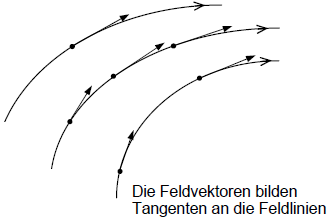
\includegraphics[width=0.2\textwidth]{pics/felder/Feldvektoren}
\end{multicols}
\subsubsection{Einige spezielle Vektorfelder}
\begin{itemize}
\begin{multicols}{2}
	\item Ein Vektorfeld heisst \textbf{homogen}, falls jedem Punkt seines Definitionsbereichs derselbe Vektor zugeordnet ist. Der Feldvektor ist also im ganzen Gebiet nach Betrag und Richtung konstant (unabhängig vom Ort). Die Feldlinien sind parallele Geraden bzw. Strecken.	
	\begin{itemize}
		\item Elektrisches Feld zwischen zwei parallelen Kondensatorplatten in
		genügend grosser Entfernung vom Rand\\
		\item Geschwindigkeitsfeld eines rein translatorisch bewegten Körpers\\
		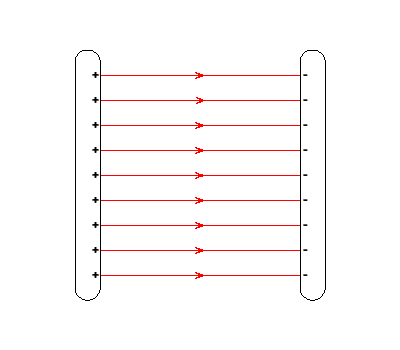
\includegraphics[width=0.15\textwidth]{pics/felder/PlattenkondensatorFeld.png}

	\end{itemize}
	\item Ein Vektorfeld heisst \textbf{eben}, falls ein rechtwinkliges Koordinatensystem so gewählt werden kann, dass alle Feldvektoren zur x-y-Ebene parallel sind und nicht von der z-Koordinate abhängen. Die Feldlinienbilder in allen Ebenen senkrecht zur z-Achse sind also identisch
	\begin{itemize}
		\item Elektrisches Feld eines Koaxialkabels (Zylindrisches Koaxialfeld)\\
		\item Elektrostatisches Feld zwischen langen, parallelen Leitern\\
		\item Magnetfeld zweier (oderer mehrerer) paralleler, gerader Leiter, die von konstanten Strömen durchflossen werden\\
	\end{itemize}
\end{multicols}
	\begin{multicols}{2}
	\item In der Elektrostatik beginnen die Feldlinien des elektrischen Feldes auf positiven Ladungen und enden auf negativen.\\
	Die positiven Ladungen können als Quellen, die negativen als Senken des elektrischen Feldes aufgefasst werden. Man spricht von einem (reinen) \textbf{Quellenfeld}.\\
		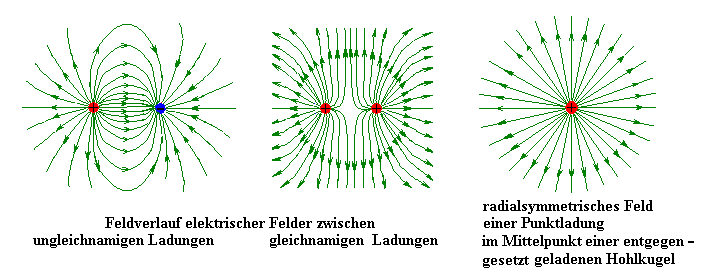
\includegraphics[width=0.5\textwidth]{pics/felder/Quellenfeld}\\
	\item Im Gegensatz zum reinen Quellenfeld steht das \textbf{Wirbelfeld}. Hier sind die Feldlinien in sich geschlossen.\\
	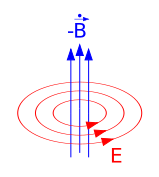
\includegraphics[width=0.2\textwidth]{pics/felder/Wirbelfeld_1}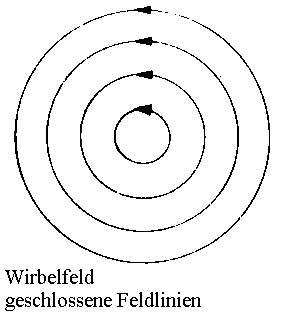
\includegraphics[width=0.2\textwidth]{pics/felder/Wirbelfeld_RotierendeScheibe}
	\end{multicols}
\end{itemize}
